\documentclass[10pt]{article}
\usepackage{graphicx}
\usepackage{listings}
\usepackage{svg}
\usepackage{xcolor}
\usepackage[margin=1.8cm]{geometry}
\usepackage{tikz}
\usetikzlibrary{arrows.meta, positioning}

\setlength{\parskip}{0.4em}
\setlength{\parindent}{0pt}

\lstset{
  basicstyle=\ttfamily\small,
  keywordstyle=\color{blue},
  commentstyle=\color{gray},
  stringstyle=\color{orange},
  frame=single,
  numbers=left,
  numberstyle=\tiny, 
  breaklines=true,
  captionpos=b
}

\title{PRAC4 : Matrix Multiplication}
\author{DIETZ T., JABER A., DONNENFELD T.}
\date{\today}

\begin{document}

\maketitle

\section{Step 1: Theoretical Analysis}

\subsection{Iterative Version: Work Partitioning}

For the classical iterative matrix multiplication, we parallelize the computation
by distributing the \textbf{rows of the output matrix} across the available threads.
Matrix multiplication has no data dependencies between rows of $C$ because:

\[
C[i,j] = \sum_{k=0}^{N-1} A[i,k]\,B[k,j],
\]

and each row of $C$ depends only on a single row of $A$ and all of $B$.

With $k$ threads, we partition rows into $k$ blocks:

\[
\text{Thread } t: 
\qquad
\text{rows } 
\frac{(t-1)N}{k}+1 
\;\text{to}\;
\frac{tN}{k}.
\]

Each thread:
\begin{itemize}
    \item reads $\frac{N}{k}$ rows of $A$,
    \item reads all of $B$,
    \item writes to disjoint rows of $C$.
\end{itemize}

This gives perfect load balance if matrix has data evenly distributed across its rows and columns and no race conditions.

\subsection{Divide and Conquer Version}

The recursive version repeatedly divides the problem into 8 independent
subproblems of size $\frac{SZ}{2}\times \frac{SZ}{2}$ until the base-case size
$DQSZ$ is reached.

Let

\[
s = \log_2\!\left(\frac{N}{DQSZ}\right)
\]

be the recursion depth.

At recursion level $i$, the number of tasks is:

\[
\text{\#tasks at level } i = 8^{\,i}.
\]

The total number of tasks is:

\[
T = \sum_{i=1}^{s} 8^{\,i}
  = \frac{8^{\,s+1} - 8}{7}.
\]

The maximum concurrency (width of the recursion tree at the deepest level) is:

\[
\text{Max concurrency} = 8^{\,s}.
\]

\subsubsection*{TikZ Task Graph Example ($N=1024$, $DQSZ=512$)}

Here $s = \log_2(1024/512)=1$, so only one level of recursion.

\begin{center}
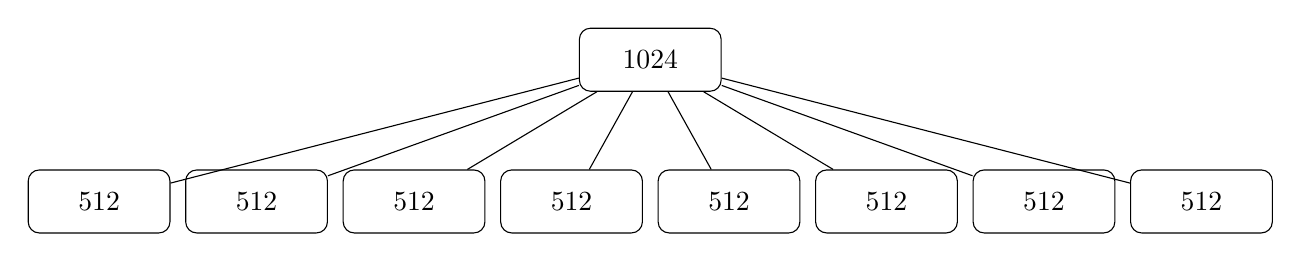
\begin{tikzpicture}[
  task/.style={rectangle,draw,rounded corners,align=center,minimum width=1.8cm,minimum height=0.8cm},
  level distance=1.8cm,
  sibling distance=2cm
]

\node[task] (root) {1024}
child { node[task]{512} }
child { node[task]{512} }
child { node[task]{512} }
child { node[task]{512} }
child { node[task]{512} }
child { node[task]{512} }
child { node[task]{512} }
child { node[task]{512} };

\end{tikzpicture}
\end{center}

\subsubsection*{$N=1024$, $DQSZ=512$}


\[
s = 1,
\qquad
T = 8,
\qquad
\text{Max concurrency} = 8.
\]

\subsubsection*{Memory Access per Task}

At each level, the 8 subproblems read and write in disjoint
quadrants of the matrices $A$, $B$, and $C$, so no task writes to the
same region of $C$.


\section{Step 2: Practical Parallel Implementation}

\subsection{Iterative Version}

We unroll the loops to take advantage of contiguous memory operations and potential SIMD vectorization.

\begin{lstlisting}[language=C++]
#pragma omp parallel for
for (int i=0; i<N; i+=2)
  for (int k=0; k<N; k+=2)
    for (int j=0; j<N; j++)
    {
      type B1 = b[k*N+j];
      type B2 = b[(k+1)*N+j];

      c[i*N+j]     += a[i*N+k]     *B1 + a[i*N+k+1]     *B2;
      c[(i+1)*N+j] += a[(i+1)*N+k] *B1 + a[(i+1)*N+k+1] *B2;
    }
\end{lstlisting}

This reduces memory accesses.

\subsection{Divide and Conquer Version}

We parallelize the recursion using OpenMP tasks:

\begin{lstlisting}[language=C++]
#pragma omp parallel
{
  #pragma omp single
  {
    #pragma omp task { ... }
    #pragma omp task { ... }
    #pragma omp task { ... }
    #pragma omp task { ... }
  }
}
\end{lstlisting}


\section{Step 3: Performance Analysis}

We benchmarked $N=2048$ for a range of thread counts and $DQSZ$ values.  
Counters collected using \texttt{perf stat}:

\begin{itemize}
    \item execution time,
    \item instructions, cycles, IPC,
    \item cache misses,
    \item speedup and efficiency.
\end{itemize}

\subsection{Heatmap 1: Execution Time}

\begin{center}
  \includesvg[width=0.90\linewidth]{./../out/time_vs_threads.svg}
\end{center}

Observations:
\begin{itemize}
    \item Large $DQSZ$ (e.g., 512–2048) yields poor performance, as the
    unblocked kernel does not fit in cache.
    \item $DQSZ=8$ or $DQSZ=16$ produce the best runtimes.
    \item These small blocks fit entirely in L1 cache and generate well-balanced
    task trees.
\end{itemize}

\subsection{Heatmap 2: Speedup (vs same-$DQSZ$, single-thread)}

\begin{center}
\includegraphics[width=0.90\linewidth]{./../out/speedup_heatmap.svg}
\end{center}

Interpretation:

\begin{itemize}
    \item Speedup is highest for small base-case sizes (8 and 16).
    \item Large $DQSZ$ values generate too few tasks, limiting parallelism.
    \item Small $DQSZ$ values enable enough fine-grained tasks to keep all
    threads busy.
\end{itemize}

\subsection{Heatmap 3: Cache Misses per Instruction}

\begin{center}
\includegraphics[width=0.90\linewidth]{./../out/cachemiss_perinst_heatmap.svg}
\end{center}

This metric highlights the core reason behind the performance trends:

\begin{itemize}
    \item Cache misses per instruction are minimal for $DQSZ=8$ and $DQSZ=16$.
    \item Their working sets fit inside L1 cache, allowing excellent locality.
    \item Larger $DQSZ$ values overflow L1/L2 and drastically increase miss rate.
\end{itemize}


\section{Step 4: Additional Optimizations}

\subsection{Loop Interchange}

Loop interchange improves spatial locality in $B$ by ensuring that inner loops
traverse memory in row-major order. This reduces cache misses for $N=2048$ and
$N=4096$.

\subsection{Register Blocking}

The 2×2 kernel retains $A$ and $B$ elements in registers long enough to compute
two output rows at a time. This greatly reduces memory bandwidth pressure.

Combined, these optimizations provide a substantial speedup for both the
iterative and recursive versions.


\section{Conclusion}

By systematically varying thread count and $DQSZ$, and by collecting hardware
performance counters, we identified the optimal configuration for matrix
multiplication on our system.

Key findings:
\begin{itemize}
    \item Small $DQSZ$ values (8 or 16) provide the best performance due to
    outstanding cache locality.
    \item Recursive task parallelism scales well when many fine-grained tasks
    are generated.
    \item Classical $DQSZ=N$ has very poor locality and serves as a worst-case
    baseline.
    \item Loop interchange and register blocking further improve performance,
    especially for large matrices.
\end{itemize}

Heatmaps proved extremely useful for visualizing how DQSZ and thread count
interact to determine performance.

\end{document}

